\section{Задача 2}

Построить область допустимых состояний многослойного композиционного материала в системе координат $\sigma_{11} - \sigma_{22} - \tau_{12}$ многослойного композиционного материала, работающего в условиях плоского напряжённого состояния. Указать характерные значения напряжений.

Схема армирования $[\phi_1 \delta_1 / \phi_2 \delta_2]$. Материал монослоёв ортотропный, технические характеристики упругости которого заданы в осях ортотропии. Модули упругости 1-го рода $E_1$ Па и $E_2$ Па, сдвиговой модуль $G_{12}$ Па, коэффициент Пуассона $\nu_{12}$ ед. Гипотеза прочности материала монослоя согласно теории максимальных нормальных напряжений. В системе координат монослоя предел прочности на растяжение в направлении 1 $F_{+1}$ Па, предел прочности на сжатие в направлении 1 $F_{-1}$ Па, предел прочности на растяжение в направлении 2 $F_{+2}$ Па, предел прочности на сжатие в направлении 2 $F_{-2}$ Па. Предел прочности на сдвиг каждого монослоя $F_{12}$ = 1 Па.

Допускается изображение области допустимого состояния многослойного композиционного материала в проекции только на одну плоскость $\sigma_{11} - \sigma_{22}$ и по наступлению предельного состояния каждого из монослоёв отдельно.

Исходные данные:
\begin{itemize}
    \item $\phi_1 = -70^\circ$
    \item $\phi_2 = 70^\circ$
    \item $E_1 = 10 \; \t{Па}$
    \item $E_2 = 4 \; \t{Па}$
    \item $\nu_{12} = 0.1$
    \item $G_{12} = 4 \; \t{Па}$
    \item $F_{+1} = 10 \; \t{Па}$
    \item $F_{-1} = -6 \; \t{Па}$
    \item $F_{+2} = 4 \; \t{Па}$
    \item $F_{-2} = -6 \; \t{Па}$
    \item $\delta_1 = 0.5$
    \item $\delta_2 = 0.5$
\end{itemize}

\subsection*{Решение}

Запишем матрицу жесткости i-го монослоя в локальной системе координат:
\begin{equation}
    \label{eq2.1}
    C_i = 
    \begin{bmatrix}
        C_{11} & C_{12} & 0
        \\
        C_{12} & C_{22} & 0
        \\
        0 & 0 & C_{33}
    \end{bmatrix}
\end{equation}

где:
\begin{equation}
    \label{eq2.2}
    C_{11} = \frac{E_1}{1 - \nu_{12} \nu_{21}}
\end{equation}
\begin{equation}
    \label{eq2.3}
    C_{22} = \frac{E_2}{1 - \nu_{12} \nu_{21}}
\end{equation}
\begin{equation}
    \label{eq2.4}
    C_{12} = \frac{\nu_{21} E_1}{1 - \nu_{12} \nu_{21}}
\end{equation}
\begin{equation}
    \label{eq2.5}
    C_{33} = G_1
\end{equation}
\begin{equation}
    \label{eq2.6}
    \nu_{21} = \nu_{12} \frac{E_2}{E_1}
\end{equation}

Тогда в глобальной системе координат матрица жесткости будет иметь вид:
\begin{equation}
    \label{eq2.7}
    C_{\Sigma i} = T_{1i} \cdot C_i \cdot T_{1i}^T
\end{equation}
где матрица перехода в глобальную систему координат $T_{1i}$ имеет вид:
\begin{equation}
    \label{eq2.8}
    T_{1i} = 
    \begin{bmatrix}
        \cos^2 \phi_i & \sin^2 \phi_i & 2 \cos \phi_i \sin \phi_i
        \\
        \sin^2 \phi_i & \cos^2 \phi_i & -2 \cos \phi_i \sin \phi_i
        \\
        - \cos \phi_i \sin \phi_i & \cos \phi_i \sin \phi_i & \cos^2 \phi - \sin^2 \phi
    \end{bmatrix}
\end{equation}

Матрицы жесткости монослоев в локальной системе координат совпадают:
\begin{equation}
    \label{eq2.9}
    C_2 = C_1 = 
    \begin{bmatrix}
        10.04 & 0.402 & 0
        \\
        0.402 & 4.016 & 0
        \\
        0 & 0 & 4
    \end{bmatrix}
    \t{Па}
\end{equation}

Получим матрицы жестости монослоев в глобальной системе координат:
\begin{equation}
    \label{eq2.10}
    C_{1\Sigma} = 
    \begin{bmatrix}
        5.004 & 0.118 & 1.306
        \\
        0.118 & 9.619 & 0.63
        \\
        1.306 & 0.63 & 3.716
    \end{bmatrix}
    \t{Па}
\end{equation}
\begin{equation}
    \label{eq2.11}
    C_{2\Sigma} = 
    \begin{bmatrix}
        5.004 & 0.118 & -1.306
        \\
        0.118 & 9.619 & -0.63
        \\
        -1.306 & -0.63 & 3.716
    \end{bmatrix}
    \t{Па}
\end{equation}

Запишем матрицы упругих податливостей монослоев для глобальной системы координат:
\begin{equation}
    \label{eq2.12}
    S_{i\Sigma} = C_{i\Sigma}^{-1}
\end{equation}
\begin{equation}
    \label{eq2.13}
    S_{1\Sigma} = 
    \begin{bmatrix}
        0.22 & 0.002 & -0.078
        \\
        0.002 & 0.105 & -0.019
        \\
        -0.078 & -0.019 & 0.3
    \end{bmatrix}
    \frac{1}{\t{Па}}
\end{equation}
\begin{equation}
    \label{eq2.14}
    S_{2\Sigma} = 
    \begin{bmatrix}
        0.22 & 0.002 & 0.078
        \\
        0.002 & 0105 & 0.019
        \\
        0.078 & 0.019 & 0.3
    \end{bmatrix}
    \frac{1}{\t{Па}}
\end{equation}

Получим матрицу жесткости для всего композиционного материала:
\begin{equation}
    \label{eq2.15}
    C_\Sigma = C_{1\Sigma} \delta_1 + C_{2\Sigma} \delta_2 = 
    \begin{bmatrix}
        5.004 & 0.118 & 0
        \\
        0.118 & 9.619 & 0
        \\
        0 & 0 & 3.716
    \end{bmatrix}
    \t{Па}
\end{equation}
и матрицу упругих податливостей:
\begin{equation}
    \label{eq2.16}
    S_\Sigma = C_\Sigma^{-1} = 
    \begin{bmatrix}
        0.2 & -0.002 & 0
        \\
        0 & 0.104 & 0
        \\
        0 & 0 & 0.269
    \end{bmatrix}
    \frac{1}{\t{Па}}
\end{equation}

Запишем соотношение для вектора напряжений в глобальной системе координат:
\begin{equation}
    \label{eq2.17}
    \{ \sigma_\Sigma \} = [C_{\Sigma}] \cdot [T_{2i}] \cdot [S_i] \cdot \left\{ \sigma_i \right\} = [K_i] \cdot \left\{ \sigma_i \right\}
\end{equation}
где матрица перехода $[T_{2i}]$ имеет вид:
\begin{equation}
    \label{eq2.18}
    T_{2i} = 
    \begin{bmatrix}
        \cos^2 \phi_i & \sin^2 \phi_i & \cos \phi_i \sin \phi_i
        \\
        \sin^2 \phi_i & \cos^2 \phi_i & - \cos \phi_i \sin \phi_i
        \\
        -2 \cos \phi_i \sin \phi_i & 2 \cos \phi_i \sin \phi_i & \cos^2 \phi_i - \sin^2 \phi_i
    \end{bmatrix}
\end{equation}

Изобразим область допустимых состояний для монослоя в локальной системе координат:
\begin{figure}[H]
    \begin{center}
        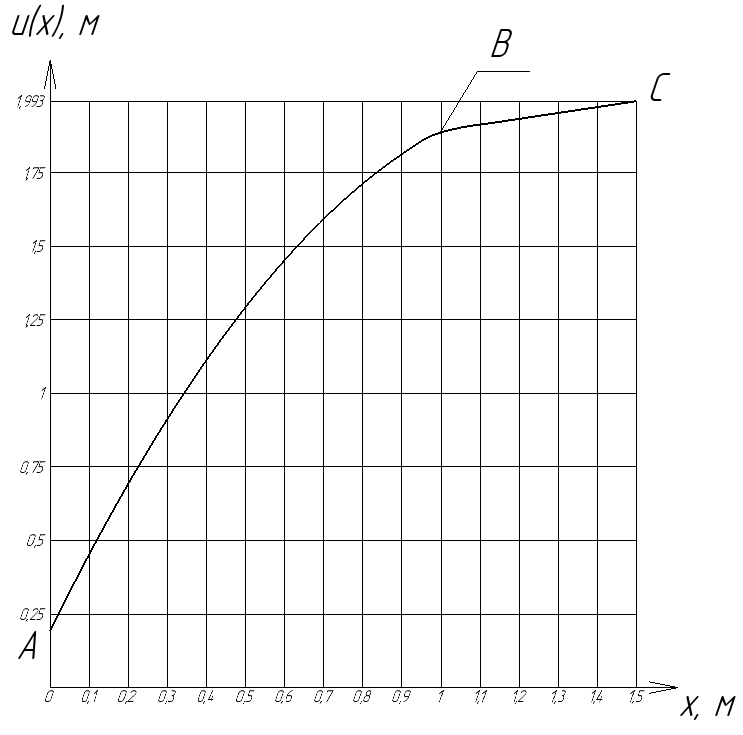
\includegraphics[width = 0.7\linewidth]{pic2.1.PNG}
        \caption{Область допустимых состояний монослоя}
        \label{pic2.1}
    \end{center}
\end{figure}

Найдем поверхность предельного состояния для всего композиционного материала:
\begin{enumerate}
\item Первый монослой:
\begin{equation}
    \label{eq2.19}
    [K_1] = [C_\Sigma] \cdot [T_{21}] \cdot [S_1] = 
    \begin{bmatrix}
        0.025 & 1.101 & -0.393
        \\
        0.838 & 0.222 & 0.763
        \\
        0.263 & -0.621 & -0.712
    \end{bmatrix}
\end{equation}
\begin{itemize}
    \item Точка $A_1$:
    \begin{equation}
        \label{eq2.20}
        \left\{ \sigma_{1A1} \right\} = 
        \begin{pmatrix}
            F_{+1}
            \\
            F_{+2}
            \\
            F_{12}
        \end{pmatrix}
        =
        \begin{pmatrix}
            10
            \\
            4
            \\
            1
        \end{pmatrix}
        \t{Па}
    \end{equation}
    \begin{equation}
        \label{eq2.21}
        \left\{ \sigma_{\Sigma A1} \right\} = 
        \begin{pmatrix}
            4.259
            \\
            10.037
            \\
            -0.568
        \end{pmatrix}
        \t{Па}
    \end{equation}
    \item Точка $A_2$:
    \begin{equation}
        \label{eq2.22}
        \left\{ \sigma_{1A2} \right\} = 
        \begin{pmatrix}
            F_{+1}
            \\
            F_{+2}
            \\
            -F_{12}
        \end{pmatrix}
        =
        \begin{pmatrix}
            10
            \\
            4
            \\
            -1
        \end{pmatrix}
        \t{Па}
    \end{equation}
    \begin{equation}
        \label{eq2.23}
        \left\{ \sigma_{\Sigma A2} \right\} = 
        \begin{pmatrix}
            5.044
            \\
            8.51
            \\
            0.855
        \end{pmatrix}
        \t{Па}
    \end{equation}
    \item Точка $B_1$:
    \begin{equation}
        \label{eq2.24}
        \left\{ \sigma_{1B1} \right\} = 
        \begin{pmatrix}
            F_{+1}
            \\
            F_{-2}
            \\
            F_{12}
        \end{pmatrix}
        =
        \begin{pmatrix}
            10
            \\
            -6
            \\
            1
        \end{pmatrix}
        \t{Па}
    \end{equation}
    \begin{equation}
        \label{eq2.25}
        \left\{ \sigma_{\Sigma B1} \right\} = 
        \begin{pmatrix}
            -6.754
            \\
            7.815
            \\
            5.642
        \end{pmatrix}
        \t{Па}
    \end{equation}
    \item Точка $B_2$:
    \begin{equation}
        \label{eq2.26}
        \left\{ \sigma_{1B2} \right\} = 
        \begin{pmatrix}
            F_{+1}
            \\
            F_{-2}
            \\
            -F_{12}
        \end{pmatrix}
        =
        \begin{pmatrix}
            10
            \\
            -6
            \\
            -1
        \end{pmatrix}
        \t{Па}
    \end{equation}
    \begin{equation}
        \label{eq2.27}
        \left\{ \sigma_{\Sigma B2} \right\} = 
        \begin{pmatrix}
            -5.969
            \\
            6.288
            \\
            7.066
        \end{pmatrix}
        \t{Па}
    \end{equation}
    \item Точка $C_1$:
    \begin{equation}
        \label{eq2.28}
        \left\{ \sigma_{1C1} \right\} = 
        \begin{pmatrix}
            F_{-1}
            \\
            F_{+2}
            \\
            F_{12}
        \end{pmatrix}
        =
        \begin{pmatrix}
            -6
            \\
            4
            \\
            1
        \end{pmatrix}
        \t{Па}
    \end{equation}
    \begin{equation}
        \label{eq2.29}
        \left\{ \sigma_{\Sigma C1} \right\} = 
        \begin{pmatrix}
            3.865
            \\
            -3.378
            \\
            -4.773
        \end{pmatrix}
        \t{Па}
    \end{equation}
    \item Точка $C_2$:
    \begin{equation}
        \label{eq2.30}
        \left\{ \sigma_{1C2} \right\} = 
        \begin{pmatrix}
            F_{-1}
            \\
            F_{+2}
            \\
            -F_{12}
        \end{pmatrix}
        =
        \begin{pmatrix}
            -6
            \\
            4
            \\
            -1
        \end{pmatrix}
        \t{Па}
    \end{equation}
    \begin{equation}
        \label{eq2.31}
        \left\{ \sigma_{\Sigma C2} \right\} = 
        \begin{pmatrix}
            4.65
            \\
            -4.905
            \\
            -3.349
        \end{pmatrix}
        \t{Па}
    \end{equation}
    \item Точка $D_1$:
    \begin{equation}
        \label{eq2.32}
        \left\{ \sigma_{1D1} \right\} = 
        \begin{pmatrix}
            F_{-1}
            \\
            F_{-2}
            \\
            F_{12}
        \end{pmatrix}
        =
        \begin{pmatrix}
            -6
            \\
            -6
            \\
            1
        \end{pmatrix}
        \t{Па}
    \end{equation}
    \begin{equation}
        \label{eq2.33}
        \left\{ \sigma_{\Sigma D1} \right\} = 
        \begin{pmatrix}
            -7.148
            \\
            -5.601
            \\
            1.438
        \end{pmatrix}
        \t{Па}
    \end{equation}
    \item Точка $D_2$:
    \begin{equation}
        \label{eq2.34}
        \left\{ \sigma_{1D2} \right\} = 
        \begin{pmatrix}
            F_{-1}
            \\
            F_{-2}
            \\
            -F_{12}
        \end{pmatrix}
        =
        \begin{pmatrix}
            -6
            \\
            -6
            \\
            -1
        \end{pmatrix}
        \t{Па}
    \end{equation}
    \begin{equation}
        \label{eq2.35}
        \left\{ \sigma_{\Sigma D2} \right\} = 
        \begin{pmatrix}
            -6.363
            \\
            -7.128
            \\
            2.862
        \end{pmatrix}
        \t{Па}
    \end{equation}
\end{itemize}
\item Второй монослой:
\begin{equation}
    \label{eq2.36}
    [K_2] = [C_\Sigma] \cdot [T_{22}] \cdot [S_2] = 
    \begin{bmatrix}
        0.025 & 1.101 & 0.393
        \\
        0.838 & 0.222 & -0.763
        \\
        -0.263 & 0.621 & -0.712
    \end{bmatrix}
\end{equation}
\begin{itemize}
    \item Точка $A_1$:
    \begin{equation}
        \label{eq2.37}
        \left\{ \sigma_{2A1} \right\} = 
        \begin{pmatrix}
            F_{+1}
            \\
            F_{+2}
            \\
            F_{12}
        \end{pmatrix}
        =
        \begin{pmatrix}
            10
            \\
            4
            \\
            1
        \end{pmatrix}
        \t{Па}
    \end{equation}
    \begin{equation}
        \label{eq2.38}
        \left\{ \sigma_{\Sigma A1} \right\} = 
        \begin{pmatrix}
            5.044
            \\
            8.51
            \\
            -0.855
        \end{pmatrix}
        \t{Па}
    \end{equation}
    \item Точка $A_2$:
    \begin{equation}
        \label{eq2.39}
        \left\{ \sigma_{2A2} \right\} = 
        \begin{pmatrix}
            F_{+1}
            \\
            F_{+2}
            \\
            -F_{12}
        \end{pmatrix}
        =
        \begin{pmatrix}
            10
            \\
            4
            \\
            -1
        \end{pmatrix}
        \t{Па}
    \end{equation}
    \begin{equation}
        \label{eq2.40}
        \left\{ \sigma_{\Sigma A2} \right\} = 
        \begin{pmatrix}
            4.259
            \\
            10.037
            \\
            0.568
        \end{pmatrix}
        \t{Па}
    \end{equation}
    \item Точка $B_1$:
    \begin{equation}
        \label{eq2.41}
        \left\{ \sigma_{2B1} \right\} = 
        \begin{pmatrix}
            F_{+1}
            \\
            F_{-2}
            \\
            F_{12}
        \end{pmatrix}
        =
        \begin{pmatrix}
            10
            \\
            -6
            \\
            1
        \end{pmatrix}
        \t{Па}
    \end{equation}
    \begin{equation}
        \label{eq2.42}
        \left\{ \sigma_{\Sigma B1} \right\} = 
        \begin{pmatrix}
            -5.969
            \\
            6.288
            \\
            -7.066
        \end{pmatrix}
        \t{Па}
    \end{equation}
    \item Точка $B_2$:
    \begin{equation}
        \label{eq2.43}
        \left\{ \sigma_{2B2} \right\} = 
        \begin{pmatrix}
            F_{+1}
            \\
            F_{-2}
            \\
            -F_{12}
        \end{pmatrix}
        =
        \begin{pmatrix}
            10
            \\
            -6
            \\
            -1
        \end{pmatrix}
        \t{Па}
    \end{equation}
    \begin{equation}
        \label{eq2.44}
        \left\{ \sigma_{\Sigma B2} \right\} = 
        \begin{pmatrix}
            -6.754
            \\
            7.815
            \\
            -5.642
        \end{pmatrix}
        \t{Па}
    \end{equation}
    \item Точка $C_1$:
    \begin{equation}
        \label{eq2.45}
        \left\{ \sigma_{2C1} \right\} = 
        \begin{pmatrix}
            F_{-1}
            \\
            F_{+2}
            \\
            F_{12}
        \end{pmatrix}
        =
        \begin{pmatrix}
            -6
            \\
            4
            \\
            1
        \end{pmatrix}
        \t{Па}
    \end{equation}
    \begin{equation}
        \label{eq2.46}
        \left\{ \sigma_{\Sigma C1} \right\} = 
        \begin{pmatrix}
            4.65
            \\
            -4.905
            \\
            3.349
        \end{pmatrix}
        \t{Па}
    \end{equation}
    \item Точка $C_2$:
    \begin{equation}
        \label{eq2.47}
        \left\{ \sigma_{1C2} \right\} = 
        \begin{pmatrix}
            F_{-1}
            \\
            F_{+2}
            \\
            -F_{12}
        \end{pmatrix}
        =
        \begin{pmatrix}
            -6
            \\
            4
            \\
            -1
        \end{pmatrix}
        \t{Па}
    \end{equation}
    \begin{equation}
        \label{eq2.48}
        \left\{ \sigma_{\Sigma C2} \right\} = 
        \begin{pmatrix}
            3.865
            \\
            -3.378
            \\
            4.773
        \end{pmatrix}
        \t{Па}
    \end{equation}
    \item Точка $D_1$:
    \begin{equation}
        \label{eq2.49}
        \left\{ \sigma_{2D1} \right\} = 
        \begin{pmatrix}
            F_{-1}
            \\
            F_{-2}
            \\
            F_{12}
        \end{pmatrix}
        =
        \begin{pmatrix}
            -6
            \\
            -6
            \\
            1
        \end{pmatrix}
        \t{Па}
    \end{equation}
    \begin{equation}
        \label{eq2.50}
        \left\{ \sigma_{\Sigma D1} \right\} = 
        \begin{pmatrix}
            -6.363
            \\
            -7.128
            \\
            -2.862
        \end{pmatrix}
        \t{Па}
    \end{equation}
    \item Точка $D_2$:
    \begin{equation}
        \label{eq2.51}
        \left\{ \sigma_{2D2} \right\} = 
        \begin{pmatrix}
            F_{-1}
            \\
            F_{-2}
            \\
            -F_{12}
        \end{pmatrix}
        =
        \begin{pmatrix}
            -6
            \\
            -6
            \\
            -1
        \end{pmatrix}
        \t{Па}
    \end{equation}
    \begin{equation}
        \label{eq2.52}
        \left\{ \sigma_{\Sigma D2} \right\} = 
        \begin{pmatrix}
            -7.148
            \\
            -5.601
            \\
            -1.438
        \end{pmatrix}
        \t{Па}
    \end{equation}
\end{itemize}
\end{enumerate}

Для каждого монослоя можно построить параллелепипед, означающий их области допустимых значений напряжений. Пересечение этих областей даст искомую область для всего композиционного материала:
\begin{figure}[H]
    \begin{center}
        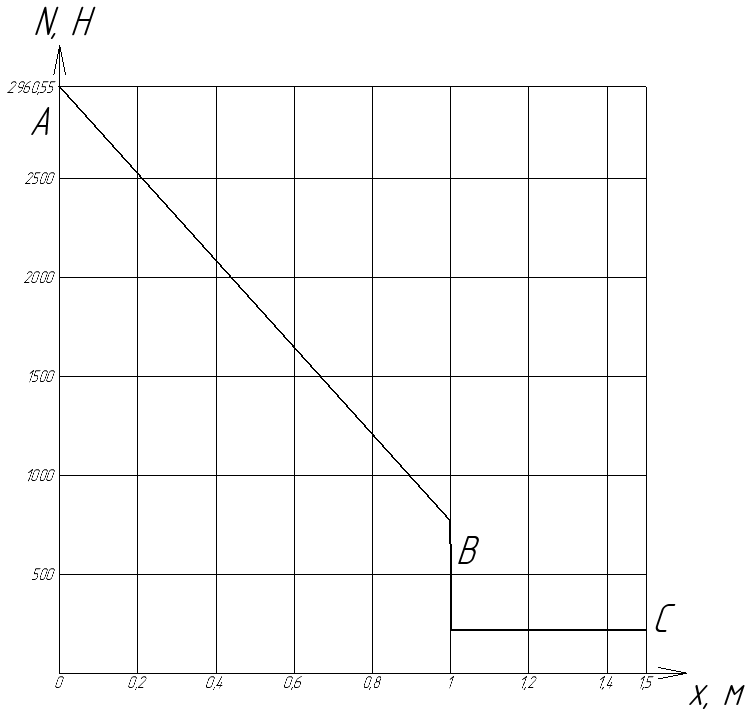
\includegraphics[width = 0.7\linewidth]{pic2.2.PNG}
        \caption{Область предельного состояния композиционного материала}
        \label{pic2.2}
    \end{center}
\end{figure}
\begin{figure}[H]
    \begin{center}
        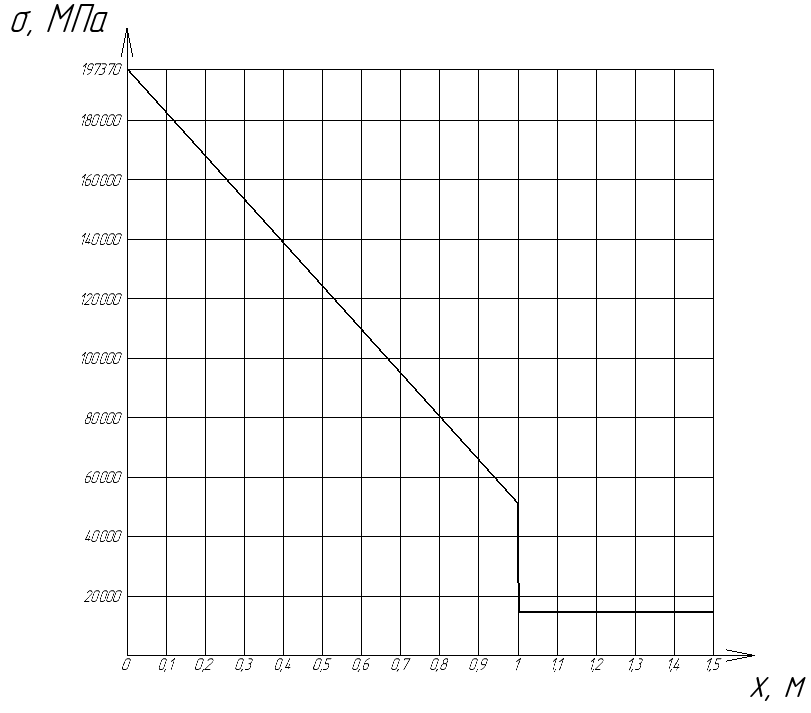
\includegraphics[width = 0.7\linewidth]{pic2.3.PNG}
        \caption{Проекция области на плоскость $\sigma_{11} - \sigma_{22}$}
        \label{pic2.3}
    \end{center}
\end{figure}